The version 1 website colour scheme is an amalgamation of white (for the background) and orange (for miscellaneous design features). The white background leverages on its simplicity and clarity, an important criteria for retaining the attention of the user. Moreover, the orange colour is reportedly stimulating for the users appetite\footnote{[ http://desktoppub.about.com/cs/colorselection/p/orange.htm ]}. The group also agreed on an orange logo design. 

\subsection{Version 1}

\begin{figure}[h]
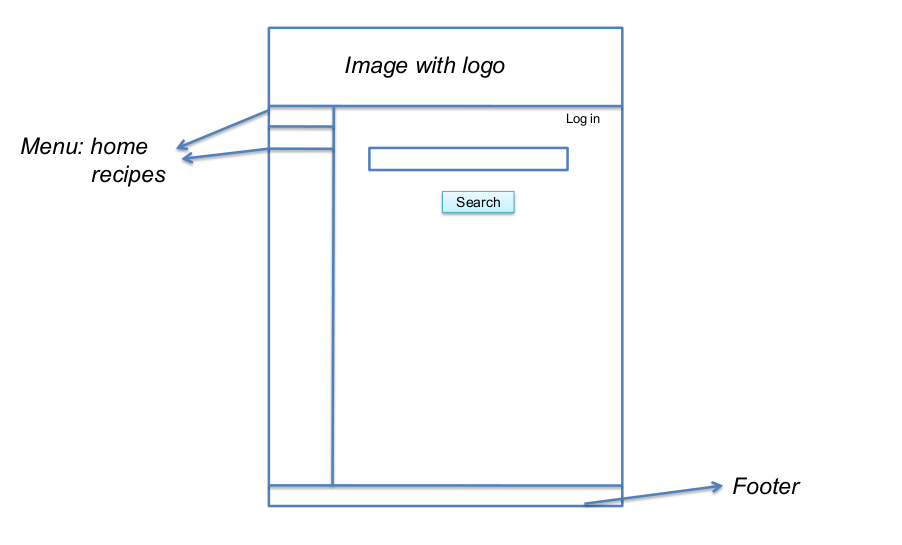
\includegraphics[width=0.9\textwidth]{home_page}
\caption{Layout of the Home Page}
\label{fig:home_page}
\end{figure}

The merit of the version 1 website design is in its simplicity. Upon accessing the website, (Fig~\ref{fig:home_page}) users are presented there are three drop-down menus which allows people to select ingredients. The drop-down menus are transversely positioned to accommodate the vertical cascading of the ingredients of the menus. Users are provided with three menus to select ingredients and submit a search. This then links to the recipe list page. Additionally, the “recipes” button in the sidebar links the page to the complete list of recipes alphabetically.

\begin{figure}[H] % Place it [H]ere, you big furry oaf! I don't care what you smell! 
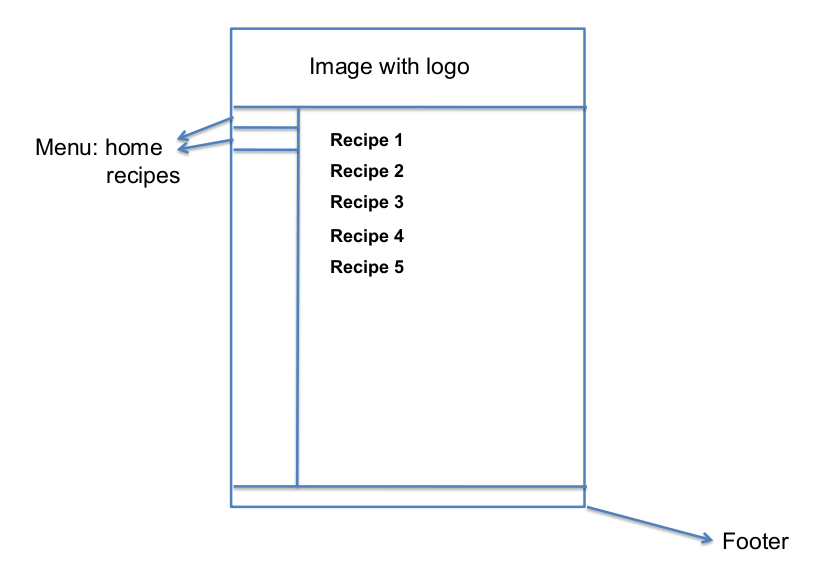
\includegraphics[width=0.9\textwidth]{recipe_list_page}
\caption{Layout of the Recipe List Page}
\label{fig:recipe_list}
\end{figure}

The recipe list page (Fig~\ref{fig:recipe_list}) contains a list of recipes with at least one of the three ingredients. However, the recipe may contain other ingredients which were not specified by the user. Upon recipe selection, the specific recipe page will be displayed.

\begin{figure}[H]
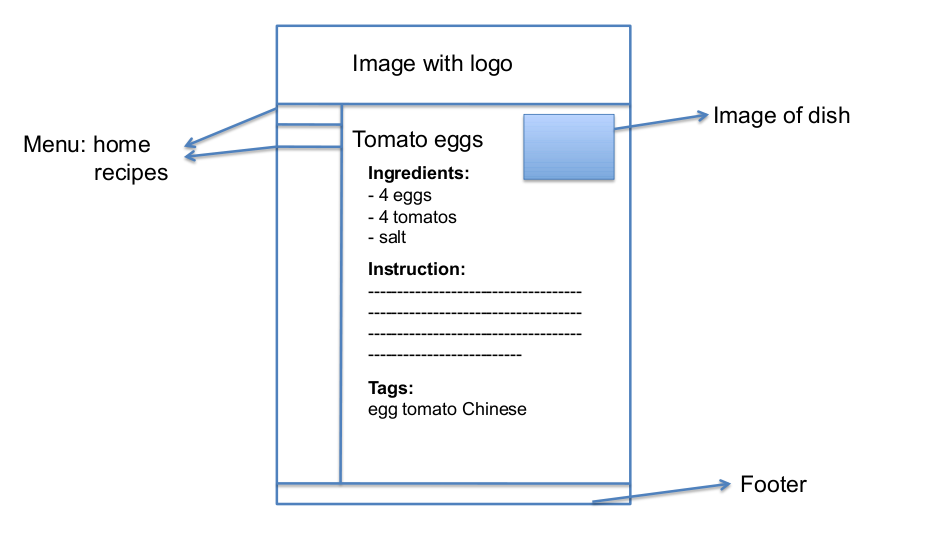
\includegraphics[width=0.9\textwidth]{recipe_page}
\caption{Layout of the Recipe Page}
\label{fig:recipe_page}
\end{figure}

The recipe page (Fig \ref{fig:recipe_page}) contains recipe details, for example recipe name, ingredients, the instruction, and recipe tags.
 
One design limitation of version 1 is that the website only has three drop-down menus, and the user is unable to type in ingredients. Being a prototype, the version 1 database is fitted with few recipes hence such functionality is redundant. 

\subsection{Version 2}
Version 2 is an upgraded version of the original version containing more functions (described by the Product Specification). With the use of technology such as JAVA Script, the web interface will look more polished. Users will be able to enter text data into ingredient selection text boxes, which will have the tab completion feature for ingredients instead of using a drop-down menu. There will also be a larger database of ingredients hence justifying the use of tab completion as apposed to drop-down menus.

Additionally, for version 2, users are allowed to have web accounts. The benefits of the account include the user having access to past recipes which he/she rated and more importantly receive recommendations of recipes they might like (this uses collaborative filtering technology). In addition, users could choose to click tags and get a list of recipes that contains that particular tag.

Additional website link may likely be created, for example a link to the most popular recipes. The website is also expected to be optimised for mobile phone viewing.

\subsection{Version 3}
The ideal version of our product involves the implementation of a variety of possible functionalities. For example, a mobile application could be developed. Recipes could be made searchable by not just ingredients but also, for instance, the type of cuisine (Chinese dish) or whether recipes are vegetarian or non-vegetarian. 

Social networking is another possibility, with users being able to interact with other users and leave comments of the pages of other users. Users might be able to upload their own recipes and receive ratings from other users. The possibility for improvements are abundant.
